% !TeX root = ../../../main.tex

The first fundamental application of the integrated pineline will actually the
inclusion of \acrfull{mhou} at \nnlo in the \nnpdfr{4.0} fit.

\pdfs are non-perturbative objects, so it may seem counter-intuitive that their
accuracy depends on perturbative series truncation.
%
This is a direct consequence of extracting them from high energy collisions
data: they are completely determined by physics that happens in the
perturbative regime, and the map discussed at the beginning of this chapter
(the one that connects data to \pdfs) is completely determined by \pqft
calculations.
%
So, the origin of the perturbative order of \pdf sets is exactly determined by
the theory predictions used during the extraction: a \nnlo set is a \pdf set
that has been fitted using theory predictions at \nnlo.
%
A \pdf set directly computed with non-perturbative methods would have no
perturbative order associated, even when used in a perturbative calculation
\footnote{
	From that point of view would be an \textit{all-order} object, even though
	it might be subject to other kinds of approximations.
}\footnote{
	Also consider that \dglap evolution is perturbative, so, once evolved, it
	acquires again a dependency on the perturbative truncation.
}.

The perturbative series enters in the \pdf in two different places: the
partonic cross section calculations (those encoded in \textit{grids}) and the
\dglap evolution\footnote{
	That technically is used twice: during the fit, to bridge data with the
	boundary condition candidate, and to evolve the final boundary condition to
	all scales.
	But considering the \pdf a function of two variables ($z$ and $\mu_F^2$)
	consistently, the abstract evolution flow used is a single one.
}.
%
In principle, these are two different perturbative orders, thus there is not a
single truncation, but two of them, and they can happen at two different
orders.
%
Still, the two objects are not completely decoupled: \dglap evolution arise
from collinear divergences, subtracted by the chosen factorization scheme.
These collinear logarithms appear as well in the partonic cross sections, so it
is important to properly account for them, avoiding double counting.
%
The whole picture of collinear subtractions is deeply connected to treatment of
quark masses, better discussed in \cref{ch:dis}, since a finite value of the
mass regulates the collinear divergence on its own.
%
Therefore, the double perturbative order already appears in the partonic cross
sections calculations, where the \fns chosen can account for light and heavy
quarks at two distinct orders (cf. \cite{Forte:2010ta}, in particular the
FONLL-B scheme).

\subsection{Estimates}
\label{sec:pine/mhou-estimate}

The goal of \mhou studies is to give an estimate of the impact of the missing
part of the perturbative series, in order to assess the size theory uncertainty
propagated on physical observables.
%
There are two categories of possible approaches: use all-order information
coming from theoretical knowledge of the perturbative series (or properties
that applies to the all-order result) and extrapolating from the behavior of
the known orders.

The first category makes use of a similar information of that consumed in
\textit{resummation}, with a different goal: resumming the perturbative series
produces a new expansion with a better convergence, while in \mhou studies the
goal is to estimate the missing part of the initial truncated series.
%
The prominent example of this category is the widespread adoption of
\textbf{scale variations} as theory uncertainties on perturbative calculations.
The physical motivation relies in Callan-Symanzik equations, the same used to
obtain \dglap (cf.\ \cref{sec:qcd/dglap}).
%
These equations encode a property of physical observables: they can not depend
on unphysical scales.
But this property holds only for the all-order physical observables, and it is
spoilt by the perturbative truncation.
Therefore, measuring the dependence of the final result on the variation of
unphysical scales, it is possible to extract the magnitude of this violation. 
%
It is not possible to reconstruct from the exact value of an observable from
this information: many missing terms do not belong to the same \textit{class}
of known ones, since it is possible to group terms in such a way that
Callan-Symanzik equations are respected for each group, but only the sum of all
groups value is the value of the full series.
%
Nevertheless, as said before the goal of \mhou investigations is not to upgrade
a truncated result to a full one, so capturing the order of magnitude is
sufficient.
%
There are cases in which the scale variations approach is known to fail, giving
an unreliable estimate also of the order of magnitude.
However, most of these cases can be predicted by simple enough properties of
the perturbative series.
E.g.\ at low enough orders some partonic channels might not be present yet,
like \dis at \lo has no gluon channel (and at \nlo no quark singlet
contribution).
%
There is not a single scale to be varied, but two: the renormalization and the
factorization scales, they have been briefly introduced in
\cref{sec:qcd/dglap}, and they also appeared in \cref{ch:dis,ch:eko}.
They are linked to the two perturbative truncations described above, so the two
of them have to be varied to obtain a complete estimate.
The way the two variations are coordinated is called a scale variations
\textit{prescription} and it is illustrated in more details in
\cref{sec:pine/mhou-scvar-note}. 

The main criticism to \textit{scale variations} is not to capture only a subset
of missing terms, that is mostly common to all approaches since the available
information is coming from the finite amount of computed terms.
Instead, it is the \textit{arbitrariness} connected to the prescriptions
themselves.
%
Even for single scale variation there is already a completely free parameter:
the amount of the variation.
%
The conventional solution, based on the logarithmic nature of the scale
dependence, is to double and halve the value of the scale, usually set to a
process scale, to minimize \enquote{spurious} contributions (but the chosen
scale is also somewhat arbitrary, for the same reason).
%
This does not solve the arbitrariness that remains in the connection between
the estimate and the real value, but it gives a way to compare the impact on
different calculations, since the two estimates will share the same arbitrary
value.

\vspace*{20pt}
\noindent
\rule{\hsize}{1pt}

\begin{itemize}
	\item Cacciari-Hudeau
	\item  Stefano's https://inspirehep.net/literature/1273674
	\item abc model https://inspirehep.net/literature/1867838
	\item MCscales https://inspirehep.net/literature/2115313)
\end{itemize} 

\subsection{Theory uncertainties in \pdf fits}
\label{sec:pine/mhou-pdf}

\begin{figure}
	\centering
	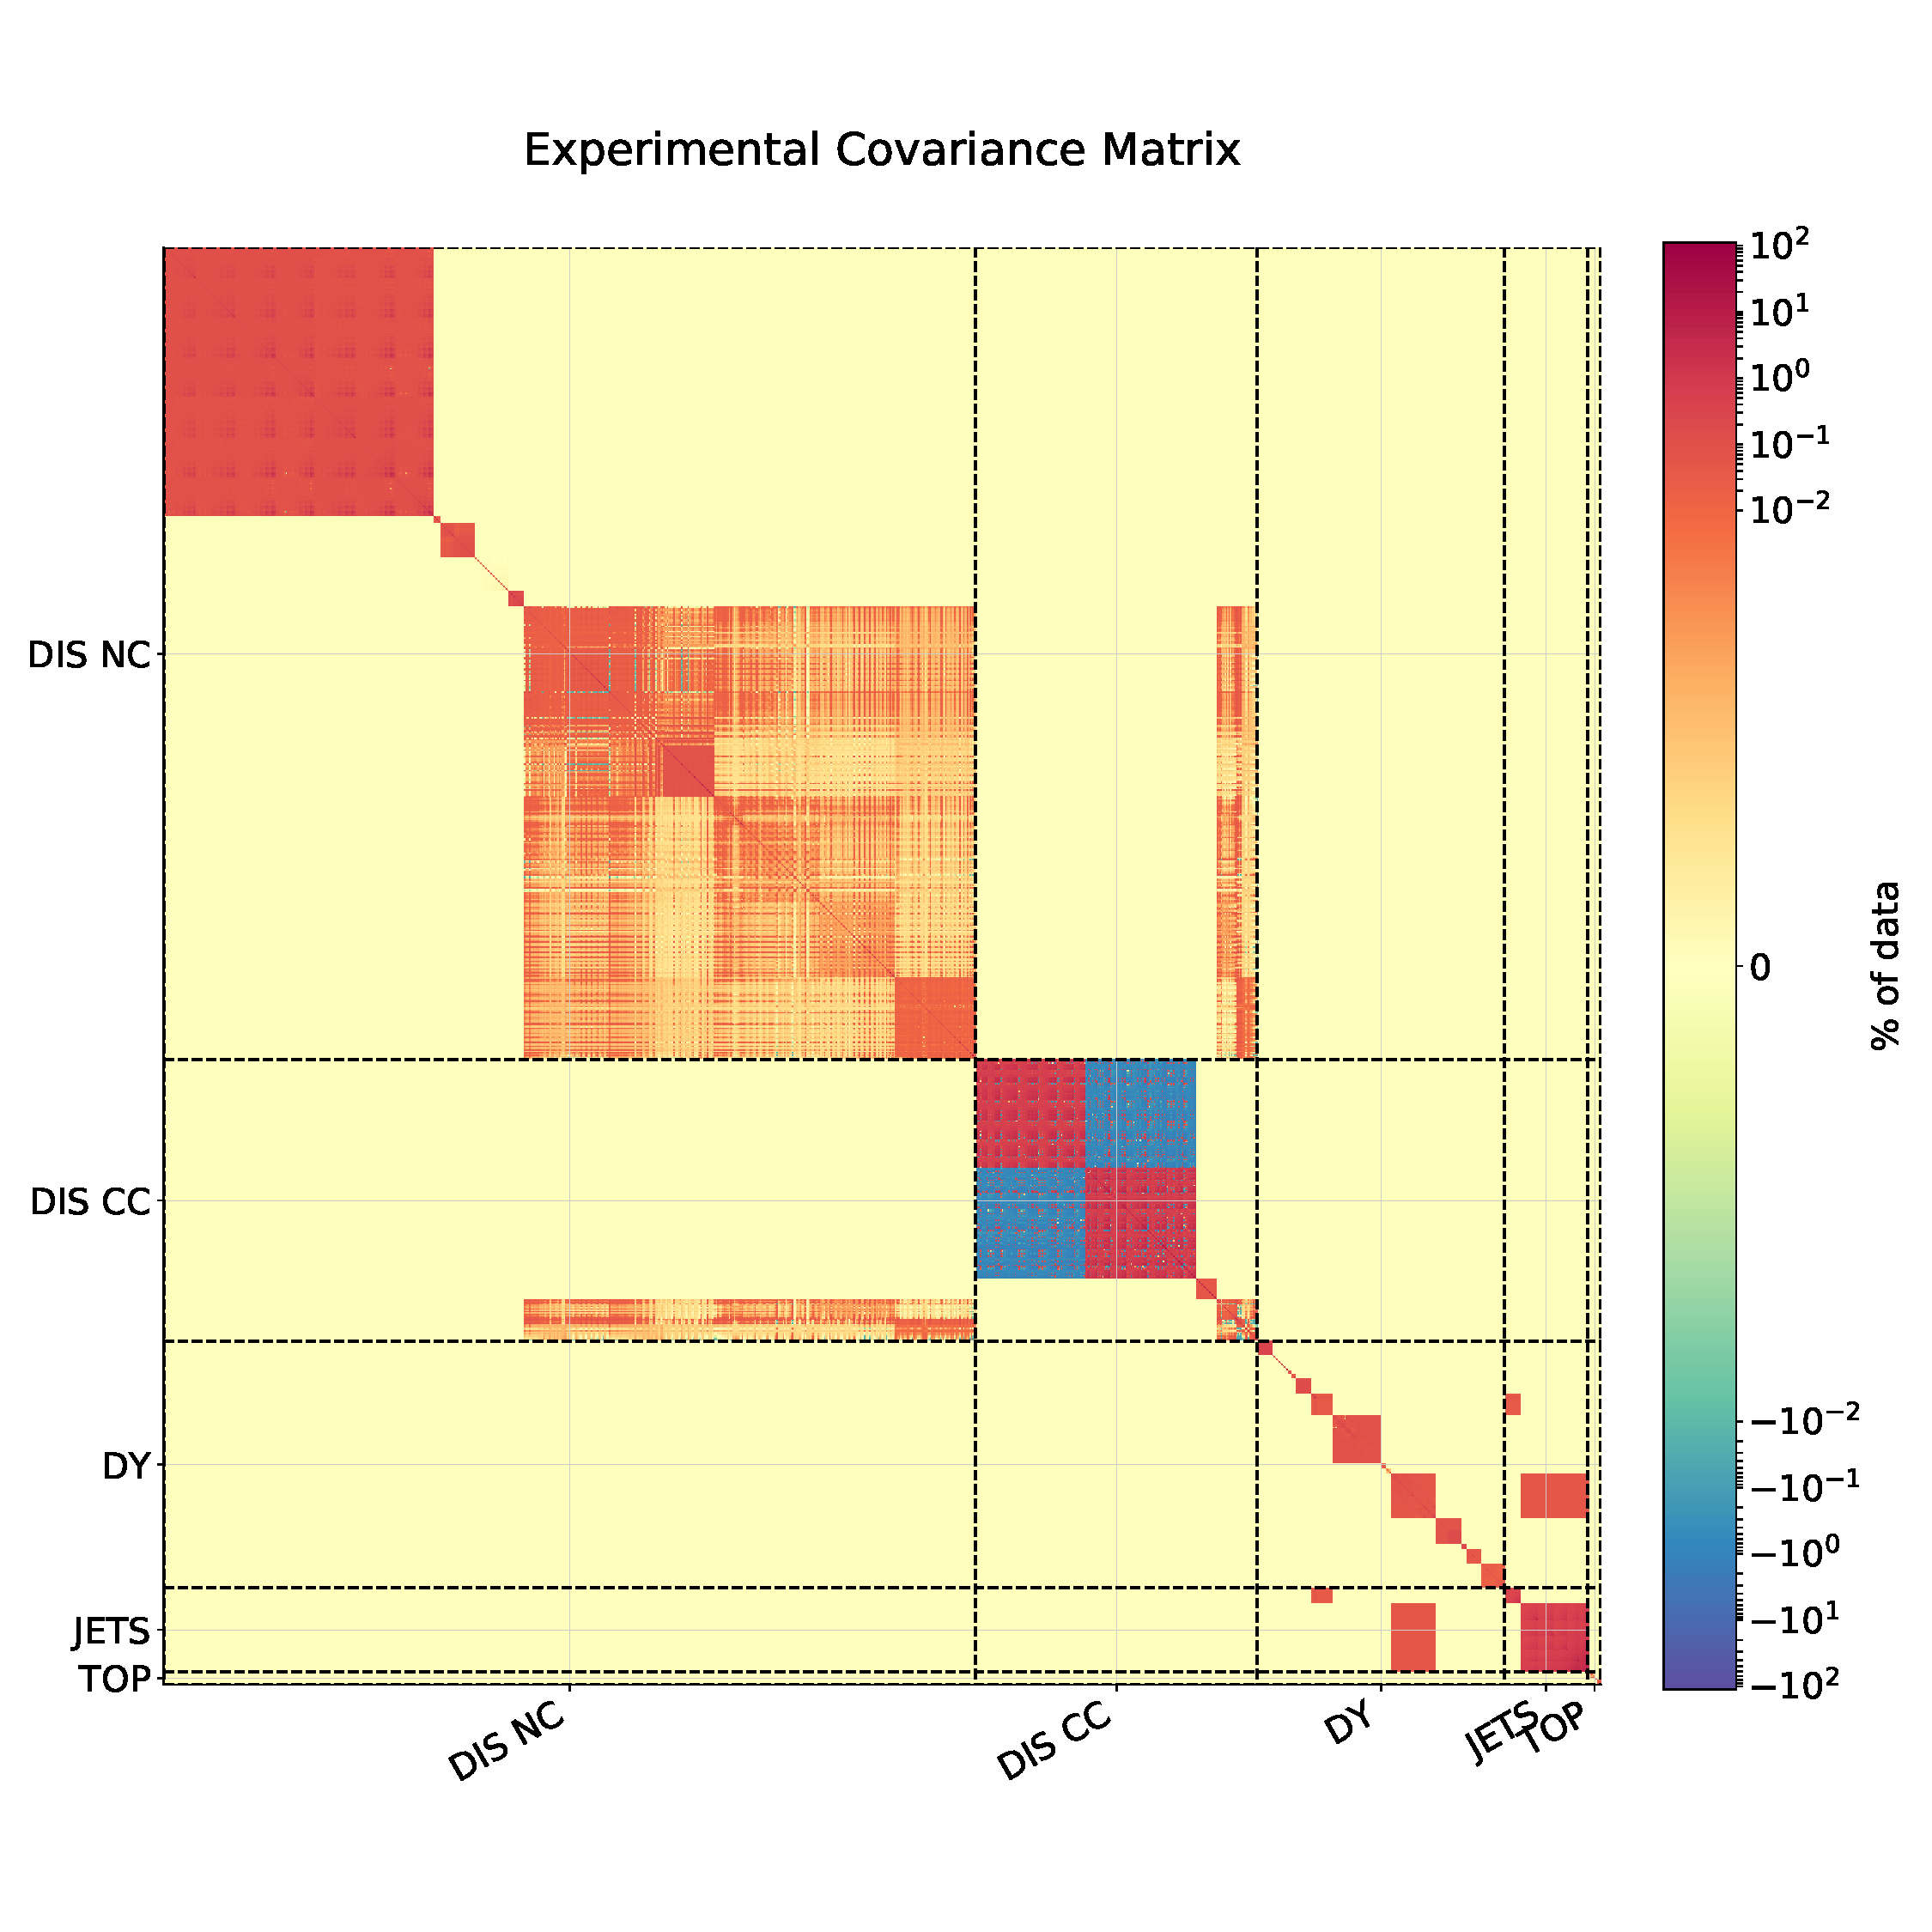
\includegraphics[width=0.49\hsize]{ch-pineline/exp_covmat}
	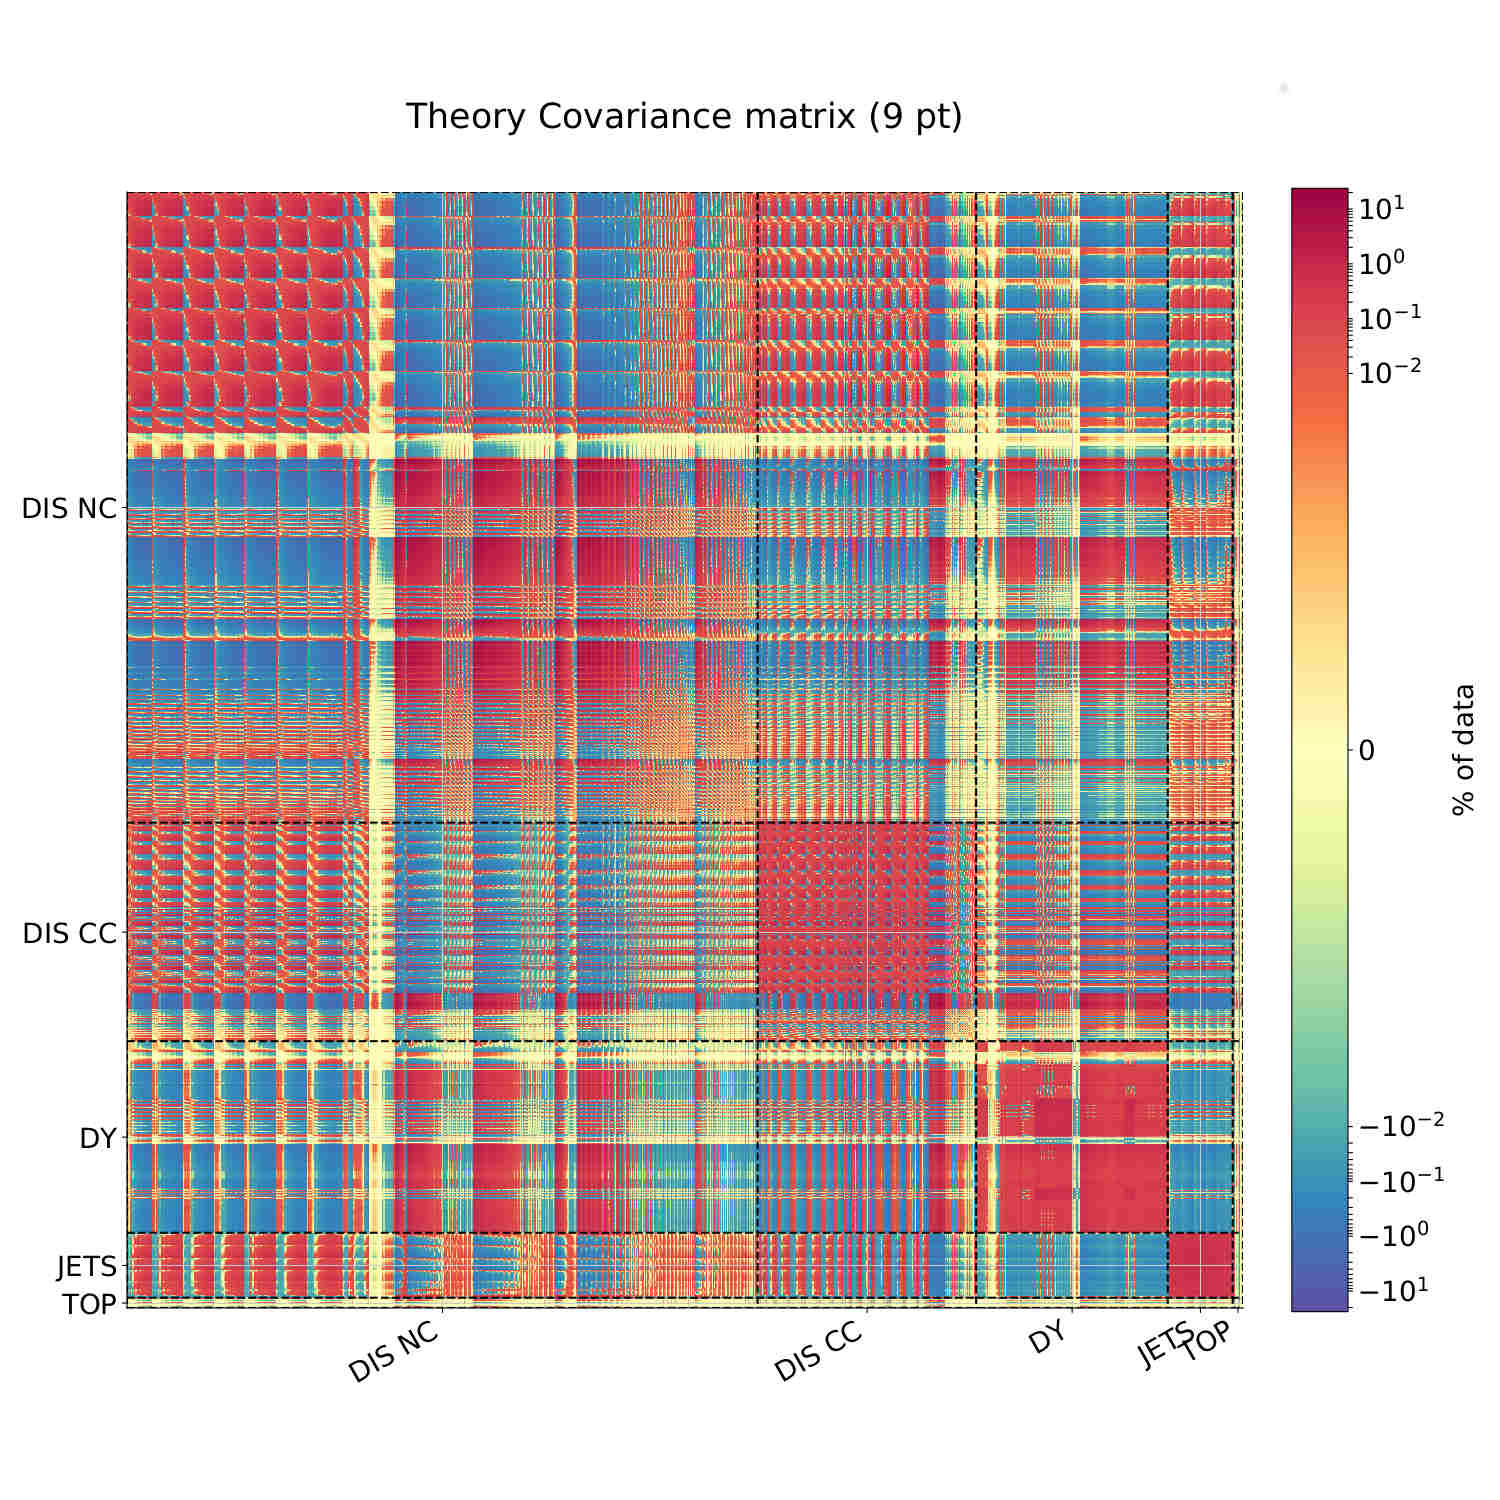
\includegraphics[width=0.49\hsize]{ch-pineline/th_covmat_9pt}
	\caption{
		Comparison between the experimental covariance matrix and the
		theoretical one, generated by the 9 point prescriptions, both
		normalized to central values.
	}
	\label{fig:pine/covmats}
\end{figure}

\begin{figure}
	\centering
	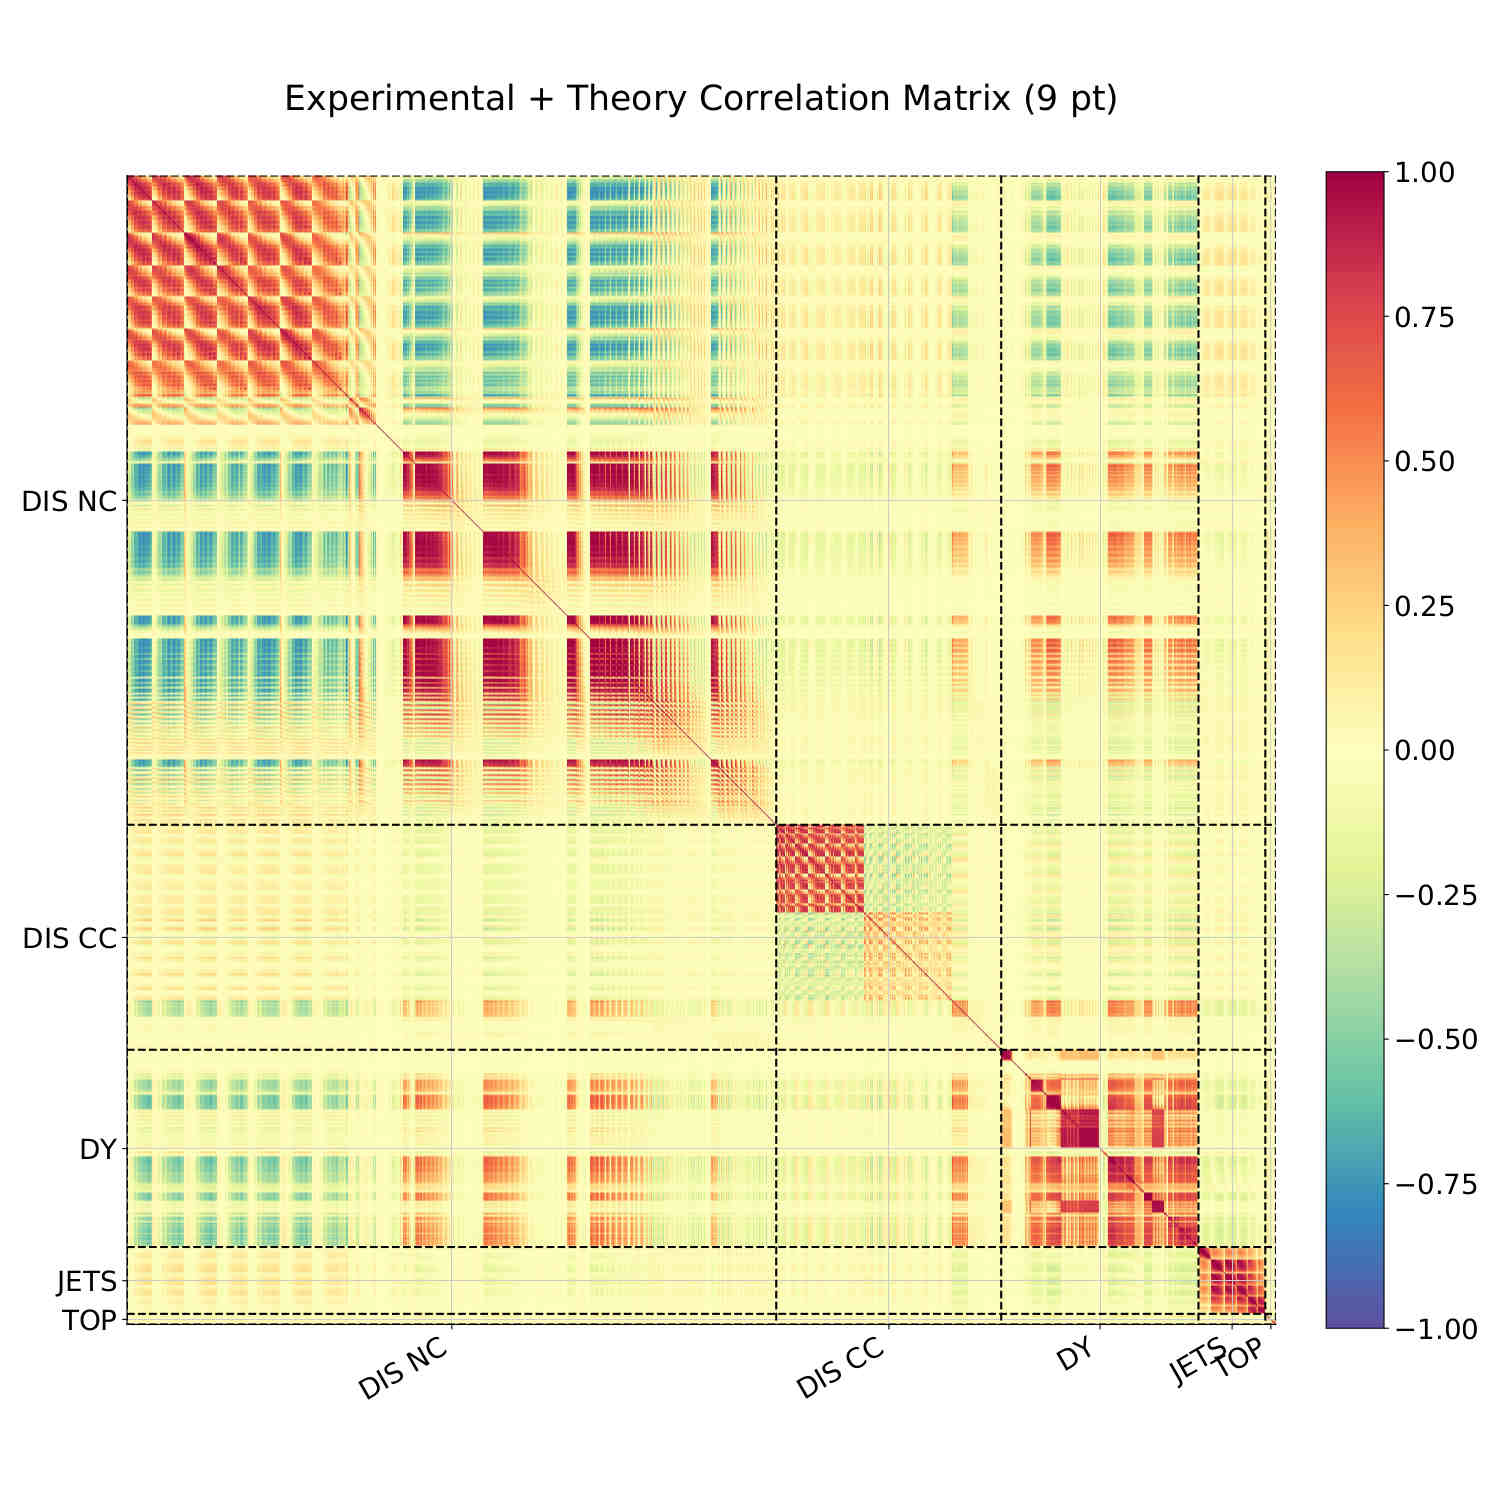
\includegraphics[width=0.7\hsize]{ch-pineline/expth_corrmat_9pt}
	\caption{
		Combined covariance matrix (experimental plus theoretical), the actual
		one used in the \nnpdfr[3.1th+]{3.1th} fit.
	}
	\label{fig:pine/combined-covmat}
\end{figure}

\begin{figure}
	\centering
	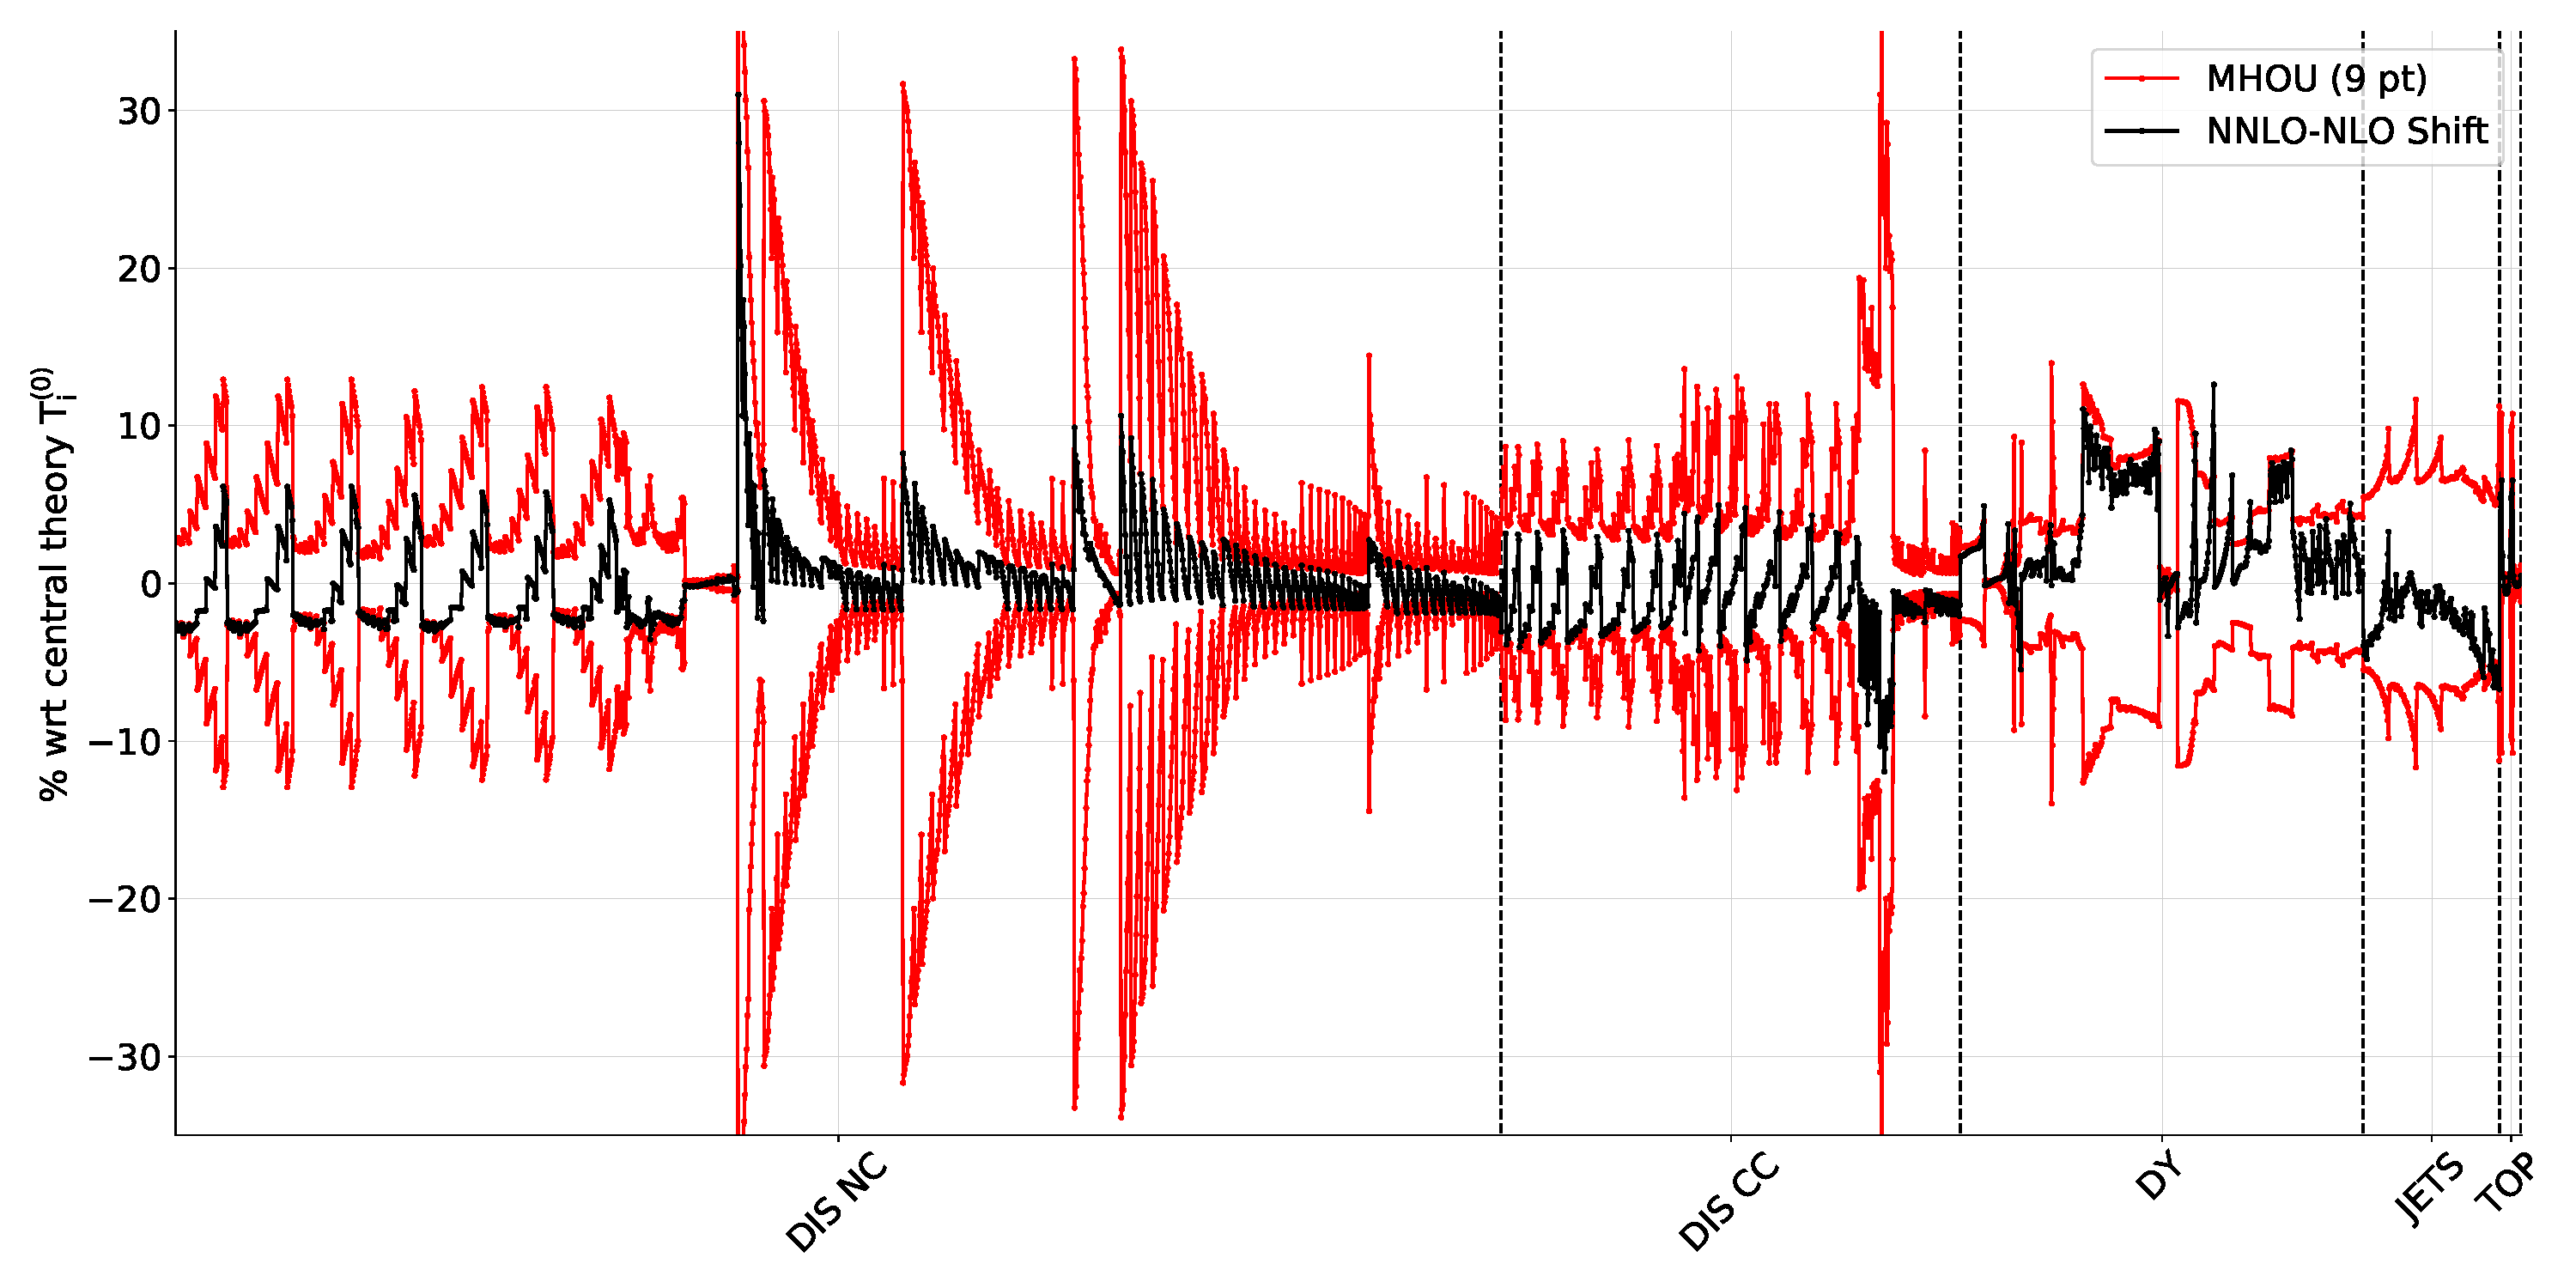
\includegraphics[width=\hsize]{ch-pineline/shift_diag_cov_comparison_9pt_global}
	\caption{
		The diagonal uncertainties $\sigma_i$ (red) symmetrized about zero,
		compared to the shift $\delta_i$ for each data-point (black).
		Values are shown as percentage of the central theory prediction
	}
	\label{fig:pine/scvar-shifts}
\end{figure}

\begin{figure}
	\centering
	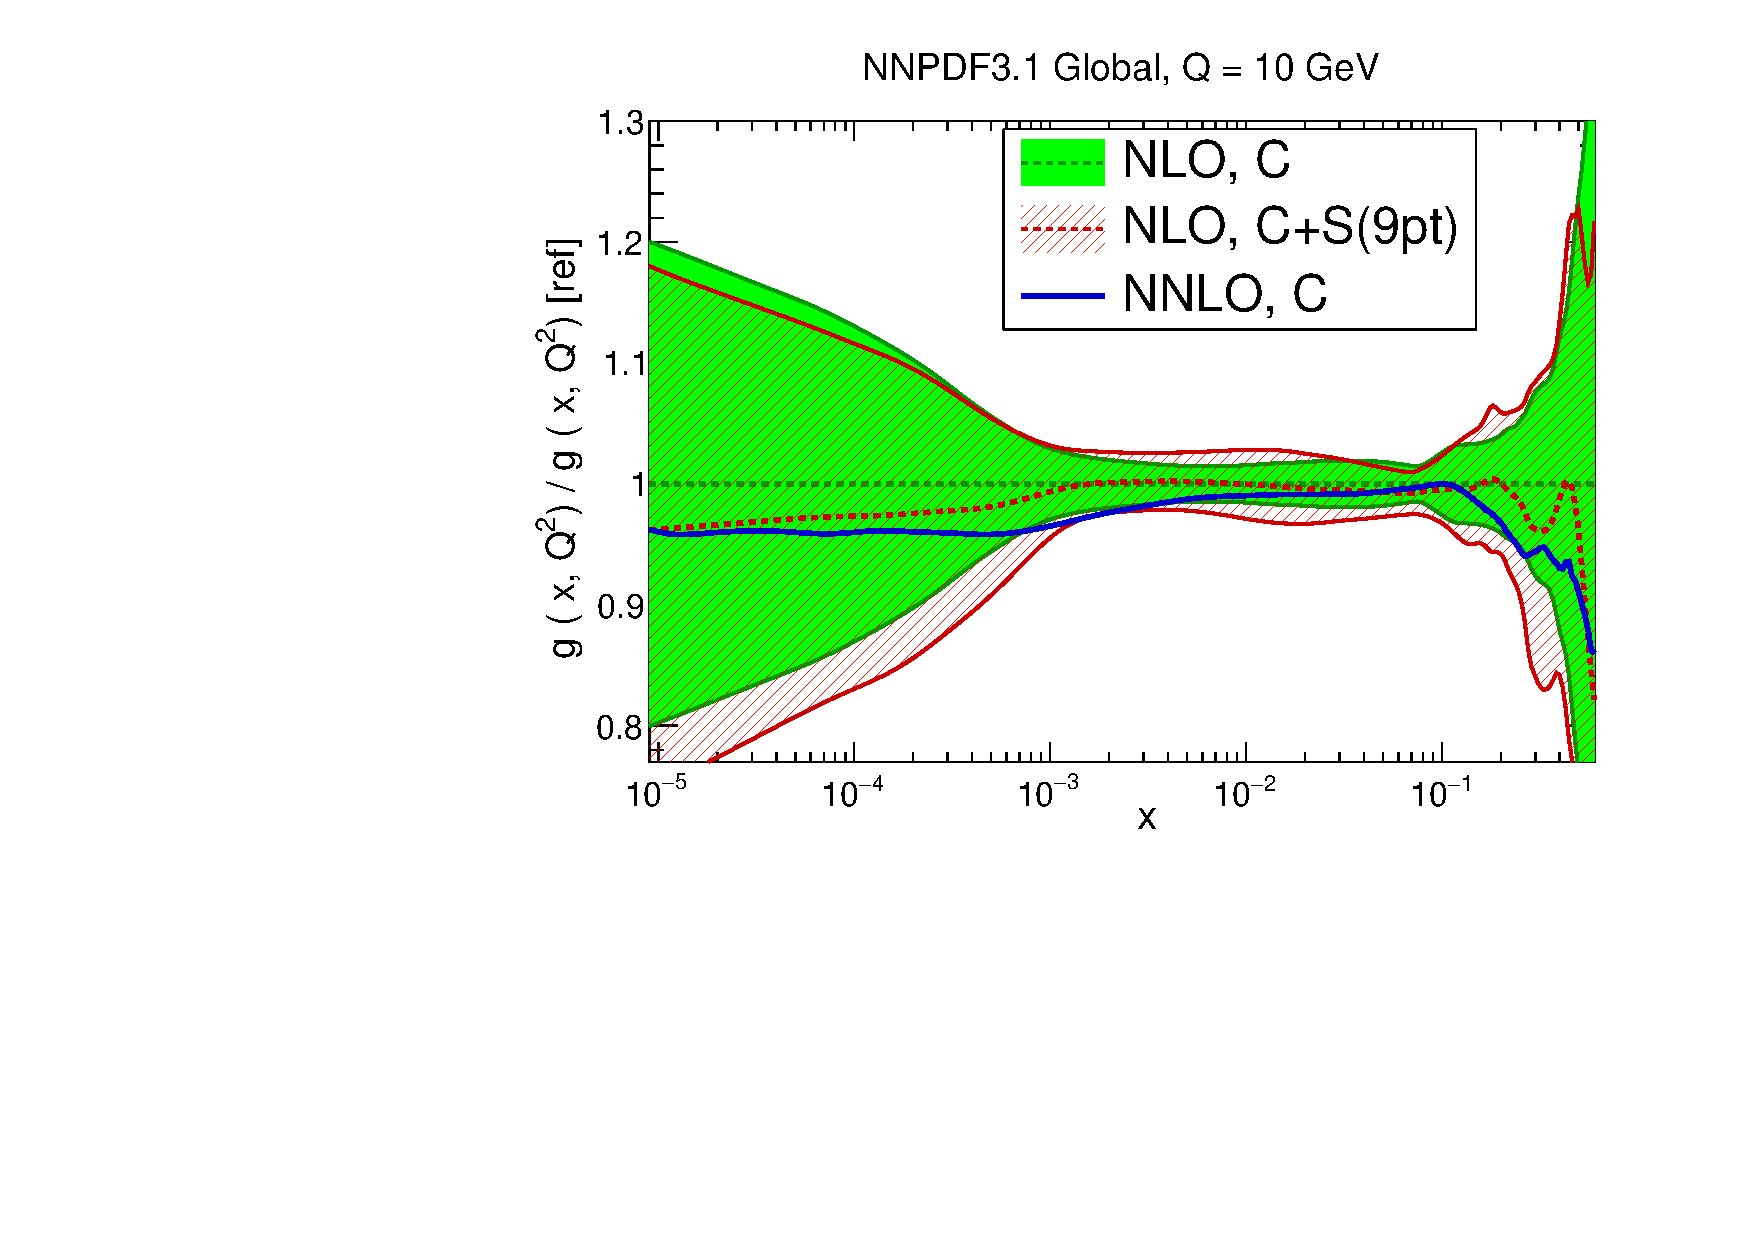
\includegraphics[width=0.49\hsize]{ch-pineline/xg-Global-NLO-CovMatTH-EXP-vsTH}
	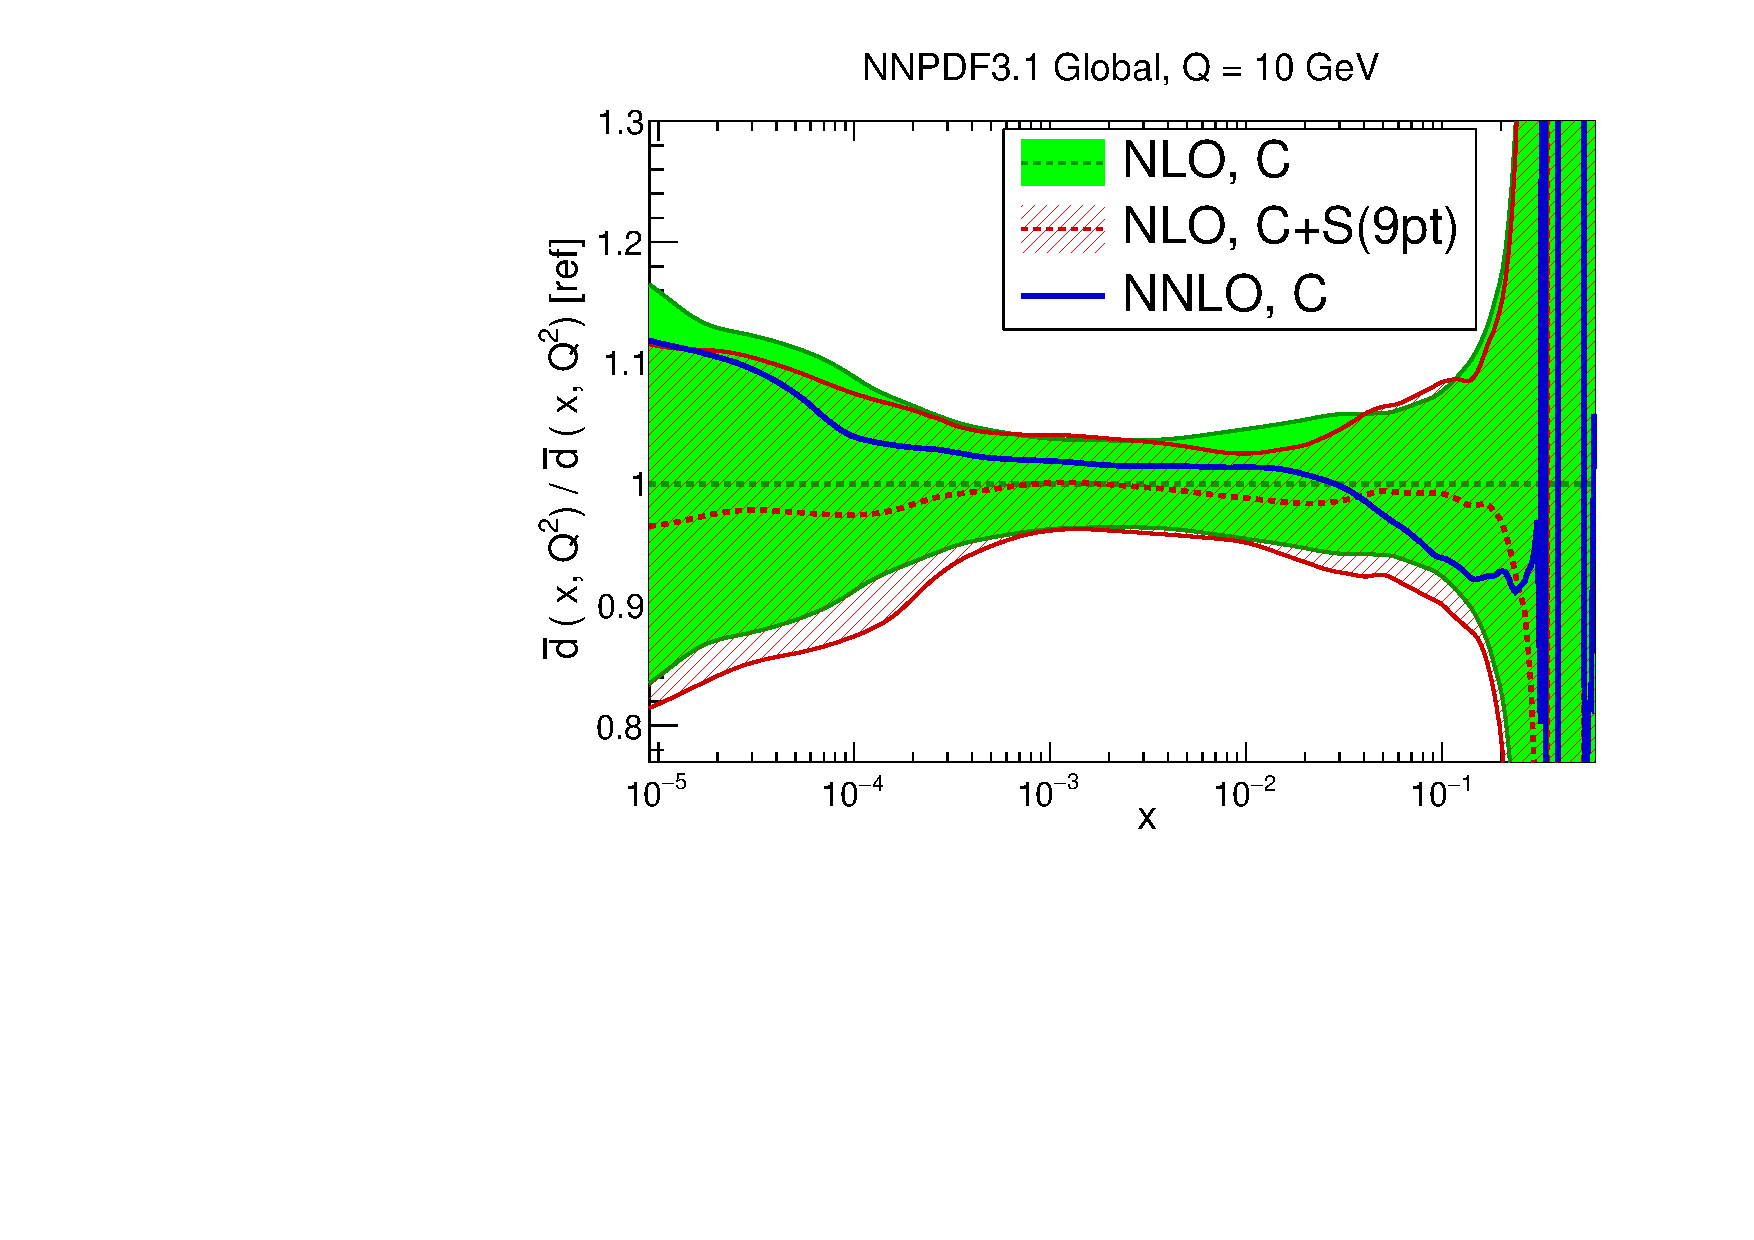
\includegraphics[width=0.49\hsize]{ch-pineline/xdbar-Global-NLO-CovMatTH-EXP-vsTH}
	\caption{
		\nnpdfr[3.1th+]{3.1th} \nlo sets, gluon and anti-down distributions at
		$\SI{10}{\giga\electronvolt}$, the first \pdf determination to include
		\mhou estimates in the fit.
	}
	\label{fig:pine/3.1th}
\end{figure}

\begin{figure}
	\centering
	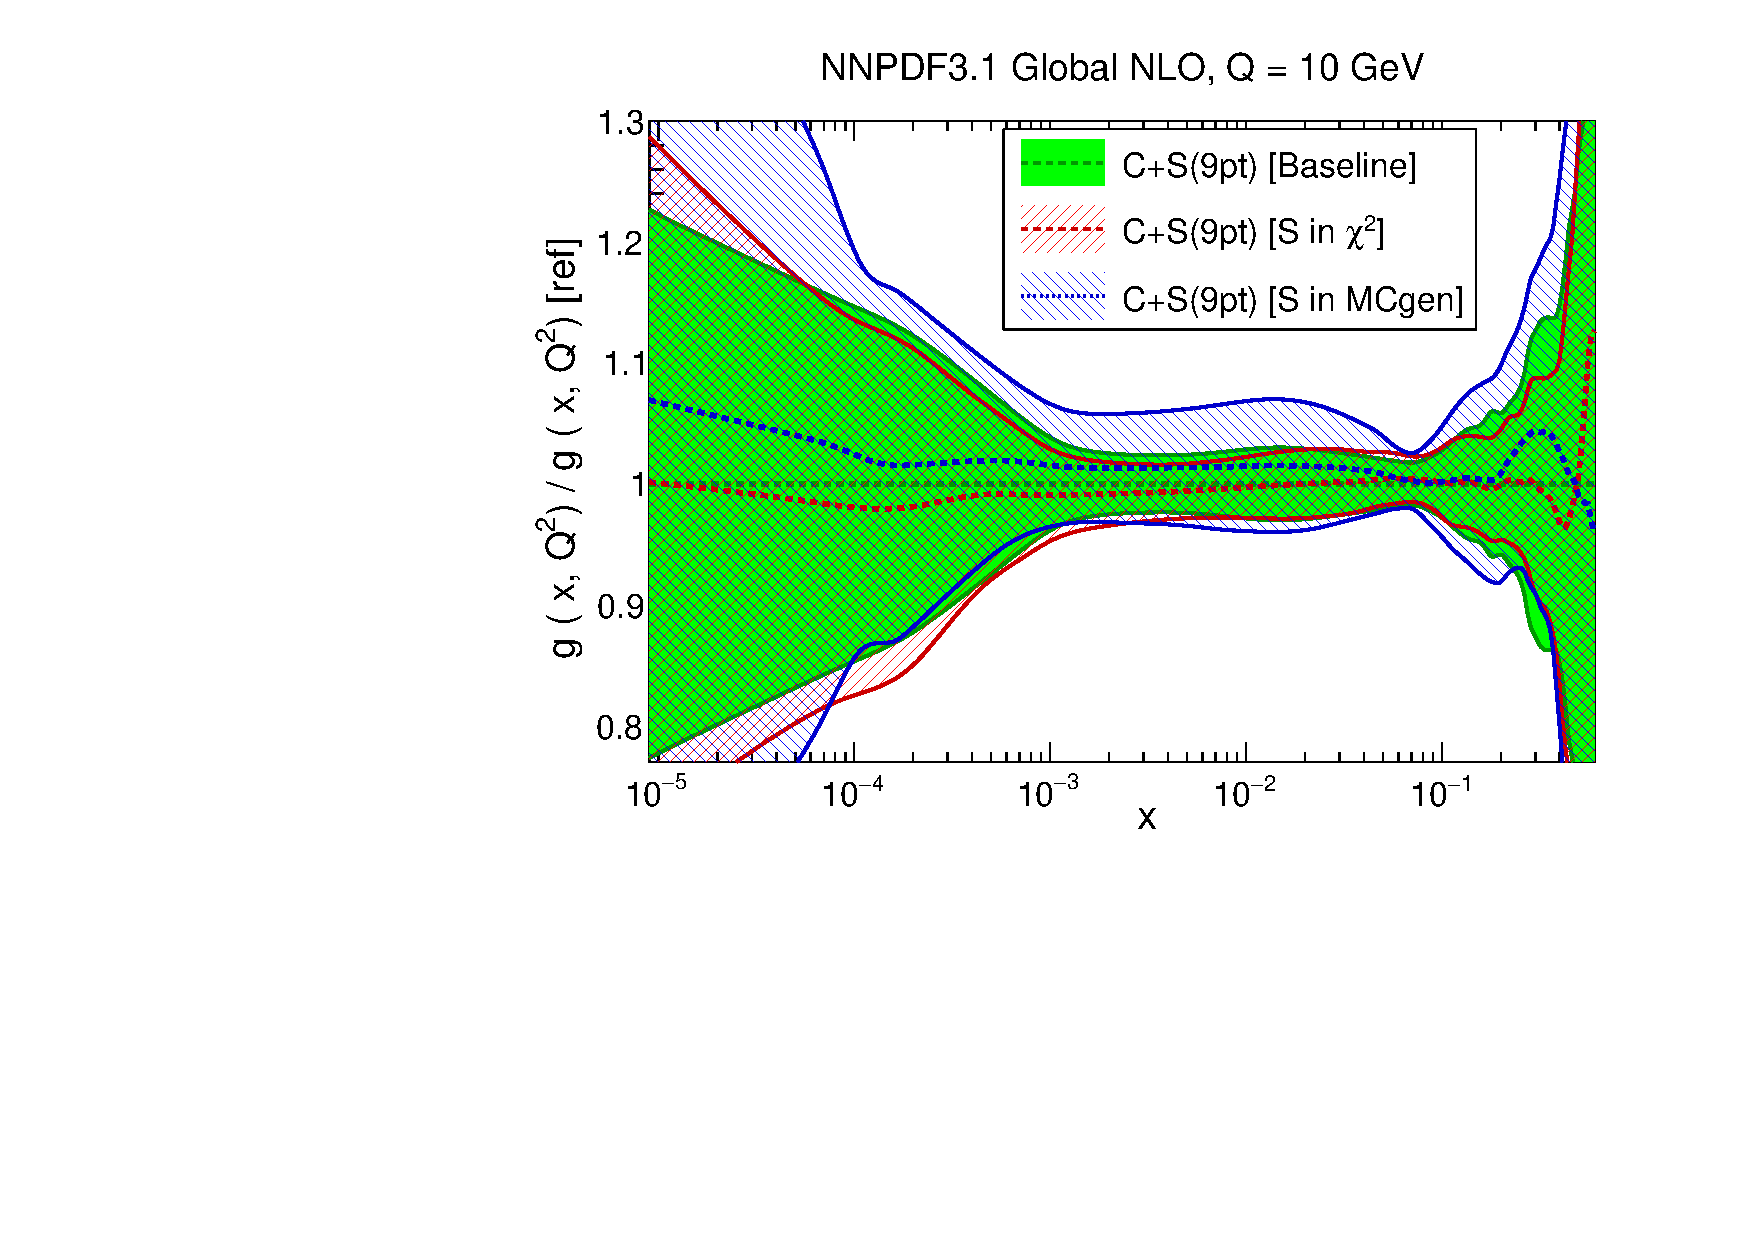
\includegraphics[width=0.49\hsize]{ch-pineline/xg-Global-NLO-CovMatTH-tests}
	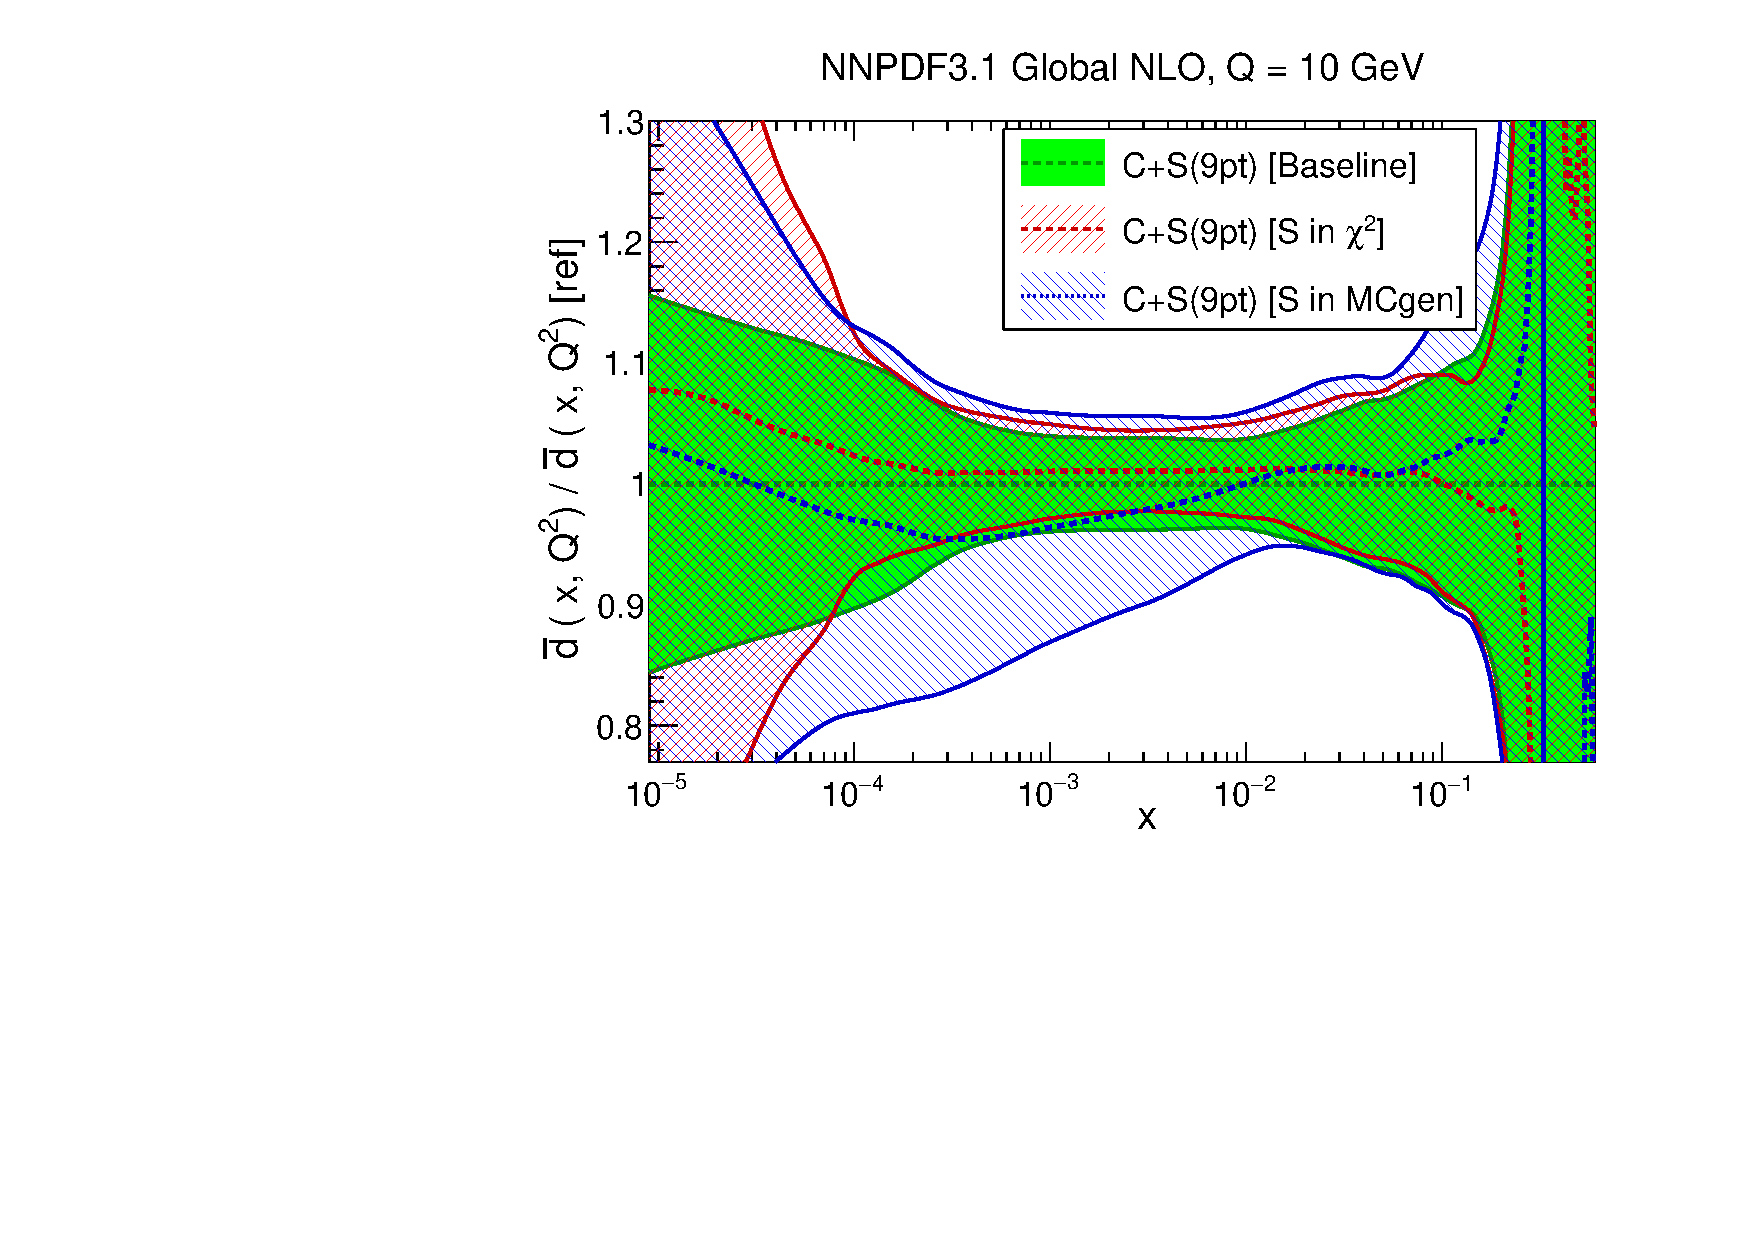
\includegraphics[width=0.49\hsize]{ch-pineline/xdbar-Global-NLO-CovMatTH-tests}
	\caption{
		Gluon and anti-down distributions comparison, in which it is shown the
		effect of using the theory covariance matrix in the $\chi^2$ or in the
		pseudo-data generation only.
	}
	\label{fig:pine/3.1th-tests}
\end{figure}


\vspace*{20pt}
\noindent
\rule{\hsize}{1pt}

\begin{itemize}
	\item brief history of MHOU in PDF fitting (cite NNPDF3.1th)
	\item theory covmat recap (take theory covmat plots from the paper)
	\item scheme B and fact scale in evolution
\end{itemize}

\subsection{New developments}
\label{sec:pine/mhou-pdf-new}

\vspace*{20pt}
\noindent
\rule{\hsize}{1pt}

\begin{itemize}
	\item actual scheme B implementation in \eko - as opposed to exponentiated
		in \apfel, i.e.\ same as \pegasus but used for B: not an issue, but it
		differs more from C, common in \mc generators
	\item what we updated wrt to NNPDF3.1th ($\alpha_s$ function vs value, and
		how ren scale vars where entering DGLAP)
	\item what is missing for a new theory covmat
	\item generate ren scale dependency in grids
\end{itemize}

\subsection{A note on scale variations prescriptions}
\label{sec:pine/mhou-scvar-note}

\vspace*{20pt}
\noindent
\rule{\hsize}{1pt}

Insert here the prescriptions note, if possible: flattened (single sections,
maybe still using \lstinline{\paragraph} for a broad subdivision) and shortened
(removing redundant or unnecessary parts).
